
\section{Experimental setup}

\subsection{Datasets}
Two public datasets were used in this study. Librispeech~\cite{librispeech}, a commonly used ASR corpus, was utilized to train the multi-modal ASR in the first stage. It consists of about 1,000 hours of 16kHz read English speech derived from read audiobooks, with the dev-clean and dev-other subsets used as the validation set, and the test-clean and test-other subsets used as the test sets. To evaluate fluency and accuracy scoring in the second stage, we conducted experiments on Speechocean762~\cite{speechocean}, an open-source speech assessment corpus consisting of 5,000 English utterances collected from 250 Chinese speakers. The whole scoring dataset is divided into 2,500 sentences for training and 2, 500 for testing. The score distribution of the test set is shown in Figure 2. The x-axis represents the human-labeled scores, and the y-axis represents the number of occurrences for each corresponding score. % 补充内容说是classess


\begin{figure}[t!]
\centering
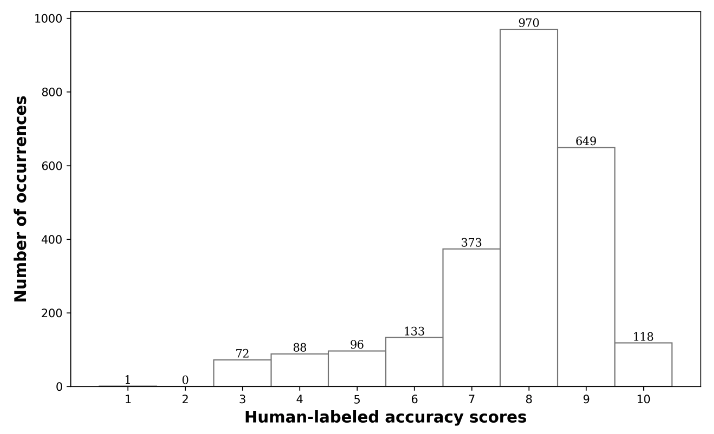
\includegraphics[width=0.35\textwidth]{content/figs/acc3.png}
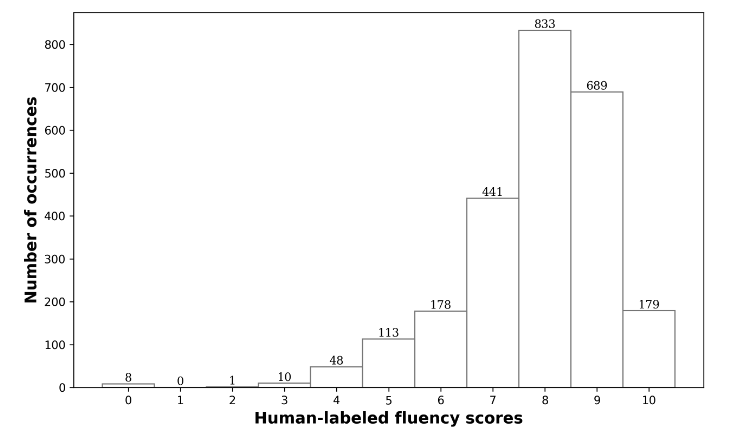
\includegraphics[width=0.35\textwidth]{content/figs/flu1.png}
\caption{The distribution of the human-labeled scores}
\label{fig: model}
\end{figure}

% \begin{figure}[t!]
% \centering
% \includegraphics[width=0.5\textwidth]{acc2.png}
% \caption{The overall pipeline for L2 learner's pronunciation assessment in the proposed system.}
% \label{fig: model}
% \end{figure}


\subsection{Setup}


% TODO
The weight of the data2vec2-based speech encoder is initialized from data2vec2-large~\footnote{\scriptsize{https://dl.fbaipublicfiles.com/fairseq/data2vec2/large\_vox\_960h.pt}} and the Qwen-based LLM~\cite{qwen} is initialized using pre-trained weights derived from Qwen-7B~\footnote{\scriptsize{https://huggingface.co/Qwen/Qwen-7B}}. For the M-adapter, we chose one MSA layer with 16 heads. The kernel size and stride of the convolution were both set to 2, aiming to halve the length of speech features extracted from the speech encoder.  

We used 8 A800s for the experiments. Each stage was trained for a maximum of two epochs on the corresponding task data. The ASR and pronunciation scoring training took about 9 and 0.2 hours, respectively. During both stages, the parameters of LLM were frozen, and the parameters of the speech encoder and modality adapter were updated. 

